\chapter{Глубокая нейросетевая модель для пространственного прогноза осадков}

\section{Сеточные данные и региональная постановка}

Во второй части работы используются сеточные региональные данные, подготовленные в формате, совместимом с бенчмарком WeatherBench~2 \cite{weatherbench2}. В отличие от станционного массива, здесь каждый объект представляет собой не вектор признаков, а пространственное поле нескольких метеорологических переменных на регулярной сетке. Это позволяет перейти от моделирования локальной точки к моделированию согласованной региональной картины осадков.

Согласно конфигурации нового ноутбука используются два основных набора данных:
\begin{enumerate}
    \item обучающий набор на сетке \(0.25^\circ\);
    \item валидационный набор 2020 года на той же сетке \(0.25^\circ\).
\end{enumerate}

Размер сетки \(0.25^\circ\) в рассматриваемом регионе равен \(159\times219\). Временной охват обучающей части составляет период с 2013-01-01 по 2019-12-29, а валидация охватывает данные 2020 года. Такое разбиение соответствует корректной временной постановке и позволяет моделировать перенос на следующий год без перемешивания временных слоев.

Для формирования входов используются инициирующие моменты с шагом 6 часов. В обучении допускаются все четыре инициализации внутри суток \(\{0,6,12,18\}\), тогда как в валидации используются инициализации \(\{0,12\}\), что согласуется с практикой регулярного прогноза. По логам подготовки данных получены:
\begin{center}
\begin{tabular}{lrr}
Набор & Число примеров & Комментарий \\
Train init & 10\,168 & последовательности для обучения \\
Validation 0.25 & 732 & выровненные валидационные запуски \\
\end{tabular}
\end{center}

\begin{table}[H]
\centering
\begin{tabular}{p{0.42\textwidth}p{0.48\textwidth}}
Параметр & Значение \\
Размер входного поля & \(159\times219\) \\
Лаги & 48, 42, 36, 30, 24, 18, 12, 6, 0 часов \\
Горизонты прогноза & 24, 48, 72, 96, 120, 144, 168, 192, 216, 240 часов \\
Число членов ансамбля & 4 \\
Базовая размерность & 64 \\
Размер окна внимания & 4 \\
Число голов внимания & 4 на первом transformer-уровне, 8 в bottleneck \\
Число эпох в конфигурации & 30 \\
Фактически сохраненная история & 12 эпох \\
Размер батча & 1 \\
Накопление градиента & 64 шага \\
Скорость обучения & \(10^{-4}\) \\
Весовая регуляризация & \(10^{-4}\) \\
Температура события при инференсе & 0.25 \\
\end{tabular}
\caption{Основные параметры региональной модели Earthformer-M в новом запуске}
\label{tab:cfg-regional-main}
\end{table}

\section{Входные и выходные тензоры модели}

На вход модели подаются динамические и статические признаки. Число динамических каналов равно 15, а число статических — 2. Динамические каналы включают метеорологические переменные на последовательности из девяти лагов:
\[
48,\ 42,\ 36,\ 30,\ 24,\ 18,\ 12,\ 6,\ 0 \text{ часов}.
\]
Следовательно, один объект имеет вид
\[
x_{\text{dyn}} \in \mathbb{R}^{9 \times 15 \times 159 \times 219}, \qquad
x_{\text{static}} \in \mathbb{R}^{2 \times 159 \times 219}.
\]
Модель должна выдать прогноз на десять горизонтов прогноза:
\[
24,\ 48,\ 72,\ 96,\ 120,\ 144,\ 168,\ 192,\ 216,\ 240 \text{ часов}.
\]
Одновременно прогнозируется несколько членов ансамбля, в конфигурации ноутбука их число равно четырем. Поэтому выходные тензоры имеют размерность
\[
\hat y_{\text{tp}} \in \mathbb{R}^{B \times 4 \times 10 \times 159 \times 219}, \qquad
\hat y_{\text{evt}} \in \mathbb{R}^{B \times 4 \times 10 \times 159 \times 219},
\]
где \(B\) — размер батча, \(\hat y_{\text{tp}}\) — логарифм прогноза осадков, а \(\hat y_{\text{evt}}\) — логиты вспомогательной вероятности экстремального события.

Важно подчеркнуть, что региональная модель решает задачу \textit{многогоризонтного} прогноза. В отличие от станционного блока, где каждый горизонт фактически рассматривается как отдельная целевая переменная в табличной модели, здесь все горизонты прогноза предсказываются общей архитектурой. Это соответствует современным подходам в нейросетевом прогнозе погоды, где одна модель захватывает общие представления и распределяет их по нескольким горизонтам прогноза.

\section{Архитектура региональной модели}

\subsection{Общая идея архитектуры}

В новом эксперименте используется модель Earthformer-M. Она заменяет предыдущий вариант региональной модели и ближе соответствует transformer-подходу к пространственно-временному прогнозу: временная ось не схлопывается сразу после входа, а сначала обрабатывается 3D-свертками и cuboid-attention блоками. Архитектура сочетает несколько идей:
\begin{enumerate}
    \item отдельную обработку динамических и статических каналов;
    \item 3D-сверточный входной тракт для сохранения временного контекста;
    \item иерархическое кодирование с ConvNeXt-блоками и cuboid transformer-блоками;
    \item temporal attention pooling перед декодером;
    \item условную выходную часть, зависящую от номера горизонта прогноза и члена ансамбля.
\end{enumerate}

Такой дизайн хорошо соответствует структуре климатических данных. Сверточные блоки эффективно обрабатывают локальные паттерны, связанные с орографией и перемещением осадочных систем, тогда как cuboid-attention блоки позволяют учитывать связи одновременно по времени и пространству. Наличие отдельных статических каналов важно для учета топографии и других неизменных характеристик региона.

\subsection{Структура входного тракта}

Динамическая часть модели начинается с двух 3D-сверток с ядром \(3\times3\times3\). Благодаря этому лаговая ось сохраняется на ранних этапах, и модель может учитывать не только отдельные карты, но и локальную эволюцию полей во времени. Это является главным отличием от более простого варианта, где временной контекст сворачивался почти сразу.

Статическая часть проходит через отдельный двумерный сверточный stem. Затем статические признаки расширяются вдоль временной оси и объединяются с динамическими признаками с помощью \(1\times1\times1\)-свертки. Такой способ слияния позволяет модели учитывать как текущее состояние атмосферы, так и неизменные особенности подстилающей поверхности.

\subsection{Кодирующая и декодирующая части}

На полном пространственном разрешении используются time-distributed ConvNeXt-блоки \cite{convnext2022}. После этого модель выполняет два уровня пространственного понижения разрешения с помощью 3D-downsample-блоков. На пониженных разрешениях применяются cuboid transformer-блоки: два блока на первом transformer-уровне и четыре блока в центральной части модели. Размер cuboid-окна по времени равен 3, а по пространственным направлениям равен \(5\times5\), поскольку он задается как \(\text{window\_size}+1\).

Перед декодером временная ось агрегируется не простым средним, а блоком temporal attention pooling. После этого декодер восстанавливает пространственное разрешение через up-блоки с пропуском признаков из кодирующей части. Первый up-блок использует гибридную структуру со вниманием, второй — сверточную обработку. Такая схема сохраняет идею U-Net \cite{unet2015}, но переносит ее в многогоризонтную пространственно-временную постановку.

\subsection{Условная выходная часть по горизонту и номеру ансамбля}

Финальный выход формируется модулем условной выходной части. Для каждого горизонта прогноза и каждого ансамблевого члена строятся embedding-представления, которые затем используются в FiLM-подобной модуляции признаков. Это важно по двум причинам.

Во-первых, разные горизонты прогноза требуют разных представлений. Ошибки на 24 часа и на 240 часов имеют разную природу, и полезно позволить модели учитывать это различие в выходном слое. Во-вторых, наличие нескольких ансамблевых членов позволяет получать не только среднее поле, но и оценивать неопределенность. В задачах детекции экстремальных осадков именно ансамблевая постановка дает возможность перейти от жесткого детерминированного решения к вероятностному прогнозу.

\section{Функция потерь и акцент на экстремумах}

В новом запуске функция потерь стала более явно ориентированной на вероятностную детекцию превышения \(q_{0.9}\). В итоговую функцию входят регрессионный Huber-loss по среднему ансамбля, квантильная функция потерь по ансамблевым членам, soft-event loss относительно локального порога, Brier-компонента и вспомогательная событийная голова:
\begin{equation}
\mathcal{L}=
0.35\mathcal{L}_{\text{tp}}+
0.45\mathcal{L}_{\text{q}}+
0.90\mathcal{L}_{\text{soft-evt}}+
0.20\mathcal{L}_{\text{Brier}}+
0.10\mathcal{L}_{\text{evt}}.
\end{equation}

Регрессионная часть удерживает физический прогноз осадков, а квантильная часть предотвращает вырождение всех ансамблевых членов в одинаковое значение. Это важно, потому что вероятность события при инференсе получается из доли членов ансамбля, превышающих локальный порог \(q_{0.9}\). Если ансамбль не разнообразен, такая вероятность становится малоинформативной.

Главная событийная компонента строится не только по вспомогательному логиту, но и по прогнозу осадков относительно карты \(q_{0.9}\):
\[
 p_{\text{soft}} = \sigma\left(\frac{\hat y_{\text{tp}}-q_{0.9}}{T_{\text{soft}}}\right),
 \qquad T_{\text{soft}}=0.35.
\]
Также используется Brier-компонента, напрямую связанная с качеством вероятностного прогноза. Для редких событий применяется focal BCE с усилением положительного класса; при этом положительный вес берется в сглаженном виде через степень \(0.5\), чтобы не переусилить редкий класс.

С методологической точки зрения это важное изменение. Обычная регрессия по осадкам склонна оптимизировать среднее качество и, следовательно, уделять чрезмерное внимание многочисленным малым или нулевым значениям. Новая функция потерь специально усиливает события около локального порога и экстремальные случаи, поэтому лучше соответствует задаче вероятностной детекции аномалий.

\section{Подготовка карт квантилей и событийных меток}

Для сеточной постановки аномалии также определяются через превышение квантиля \(q_{0.9}\), но порог хранится в виде \textit{карты} для каждой ячейки сетки. Это означает, что экстремальность определяется локально по каждой ячейке. Такой подход необходим, поскольку распределение осадков неоднородно по региону: морские области, горные районы и континентальные зоны имеют разные характерные уровни и дисперсии. Локальная карта порогов делает критерий аномальности физически и статистически осмысленным.

\begin{figure}[H]
    \centering
    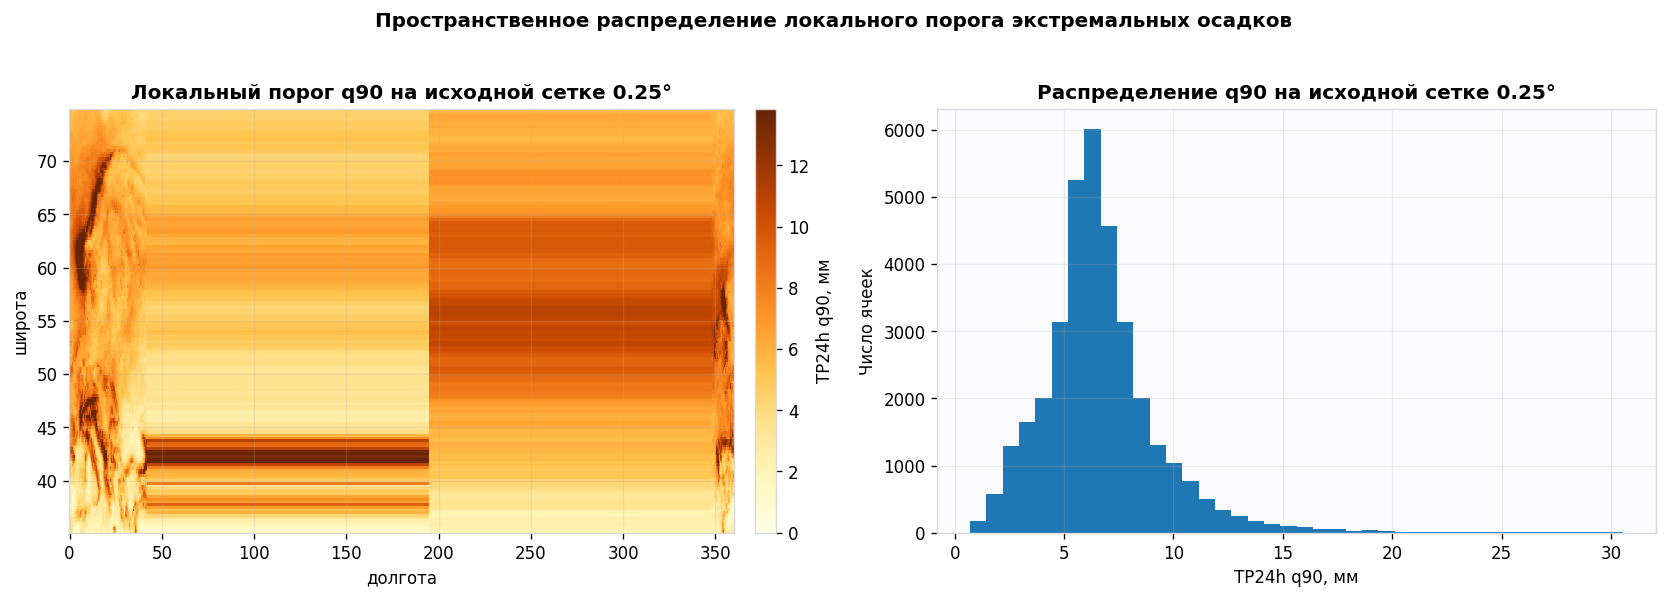
\includegraphics[width=0.95\textwidth]{figures/notebook/15_q90_threshold_maps.png}
    \caption{Пространственное распределение локального порога \(q_{0.9}\) для определения экстремальных осадков. На рисунке показано, что один общий порог для всего региона был бы слишком грубым приближением.}
    \label{fig:q90-threshold-maps}
\end{figure}

На рисунке~\ref{fig:q90-threshold-maps} видно, что порог экстремальности заметно меняется по пространству. Поэтому я не использую единый абсолютный порог осадков для всего региона: одно и то же значение суточной суммы может быть нормальным для влажной горной или прибрежной области и одновременно аномальным для более сухой континентальной зоны. Такой способ задания события делает дальнейшие метрики более честными по отношению к климатическим различиям внутри области.

Итоговые метрики считаются не только для вспомогательной головной части события, но и для вероятностной интерпретации прогноза \(\mathrm{TP24h}\) относительно локального порога. Такое решение согласуется с логикой вероятностной оценки гидроклиматического события, где основное внимание уделяется качеству прогнозируемого гидроклиматического события, а не только внутреннему сигнальному каналу модели.

\section{Ресурсные ограничения и инженерные аспекты обучения}

Еще одной важной частью исследования является учет вычислительных ограничений. Новый запуск выполнялся в среде Colab на графическом процессоре Tesla T4. Поэтому фактическая конфигурация была уменьшена относительно более тяжелого варианта: базовая размерность равна 64, размер батча равен 1, а число шагов накопления градиента равно 64. Это позволяет обучать модель на сетке \(0.25^\circ\), сохраняя полный набор горизонтов и четыре ансамблевых члена.

Также включена gradient checkpointing, которая уменьшает использование памяти ценой дополнительного времени вычисления. Этот аспект не является второстепенным: в задачах климатического глубокого обучения инженерная реализуемость модели часто столь же важна, как и ее теоретическая выразительность.

В логах обучения явно контролируется численная устойчивость: проверяются значения \texttt{NaN} и \texttt{Inf} во входных данных, статистиках нормировки, параметрах модели и промежуточных предсказаниях. Такое внимание к диагностике особенно важно в задачах осадков, где распределение целевой переменной резко асимметрично и может провоцировать нестабильность при переходе к логарифмическому пространству или при работе с экстремальными случаями.

\section{Почему для этой постановки нужна именно глубокая модель}

Теперь можно ответить на принципиальный вопрос: почему вторая часть работы не ограничивается табличными алгоритмами, а требует глубокой нейросетевой архитектуры?

Во-первых, вход имеет высокую размерность и естественную пространственную топологию. Если развернуть поле \(159\times219\) по всем каналам и лагам в один вектор, размерность станет чрезвычайно большой, а локальная структура будет уничтожена. Сверточные и transformer-блоки позволяют использовать эту структуру напрямую.

Во-вторых, задача требует согласованного прогноза на нескольких горизонтах прогноза и по нескольким ансамблевым членам. Табличный подход скорее привел бы к набору независимых моделей, каждая из которых не использовала бы общие представления процесса. Глубокая модель, наоборот, естественно извлекает общее скрытое представление и далее специализирует его по горизонту.

В-третьих, детекция аномалий в климатических полях зависит не только от значения в одной ячейке, но и от окружающего контекста: формы осадочной системы, орографического усиления, фронтальных структур, адвекции влаги. Такие зависимости трудно выразить через ручные признаки, но именно они являются сильной стороной глубоких сетей.

Наконец, глубокая модель позволяет объединить в одной архитектуре регрессию по сумме осадков и вспомогательную задачу событийного прогнозирования. Это делает постановку ближе к реальному сценарию риск-ориентированного прогнозирования, когда пользователю важны и ожидаемая интенсивность, и вероятность опасного эпизода.

\section{Промежуточные выводы}

Таким образом, сеточная часть работы формирует полноценную глубокую постановку задачи. Региональная модель Earthformer-M получает на вход многоканальные последовательности полей, сохраняет временной контекст в 3D-сверточном тракте, использует cuboid transformer-блоки на пониженных разрешениях, обучается на комбинации регрессионных и событийных функций потерь и оценивается на валидационном периоде 2020 года. В следующей главе будет показано, как результаты этой модели соотносятся с базовой постановкой, какие качественные закономерности проявляются в метриках и что можно сказать о способности модели выделять экстремальные осадочные события на основе доступных экспериментальных логов.
